%% shor_presentacion.tex
%% Presentación: El Algoritmo de Shor
%% Materia: Computación Cuántica — ITBA
%% Compilar: bash ~/.claude/skills/latex-document/scripts/compile_latex.sh shor_presentacion.tex --use-latexmk

\documentclass[aspectratio=169]{beamer}

%% ── Codificación e idioma ──────────────────────────────────────────────────
\usepackage[utf8]{inputenc}
\usepackage[T1]{fontenc}
%% (babel Spanish puede no estar disponible en esta instalación — se omite)

%% ── Matemática ─────────────────────────────────────────────────────────────
\usepackage{amsmath, amssymb}
\usepackage{physics}        % \ket, \bra, \braket, \mel, etc.

%% ── Gráficos y circuitos ───────────────────────────────────────────────────
\usepackage{tikz}
\usetikzlibrary{shapes.geometric, arrows.meta, positioning, calc}
\usepackage{quantikz}   % quantum circuit diagrams

%% ── Tablas ─────────────────────────────────────────────────────────────────
\usepackage{booktabs}
\usepackage{colortbl}

%% ── Tipografía / layout ────────────────────────────────────────────────────
\usepackage{xcolor}
\usepackage{hyperref}

%% ── Tema ───────────────────────────────────────────────────────────────────
\usetheme{metropolis}

%% ── Colores del proyecto ───────────────────────────────────────────────────
\definecolor{clasico}{RGB}{0,70,140}    % azul  — pasos clásicos
\definecolor{cuantico}{RGB}{180,80,0}   % naranja — el único paso cuántico
\definecolor{alerta}{RGB}{180,30,30}    % rojo   — modo de fallo

%% ── Estilos TikZ (diagramas de flujo) ─────────────────────────────────────
\tikzset{
  clbox/.style={rectangle, draw=clasico, fill=clasico!10, rounded corners=3pt,
                text width=8cm, align=left, font=\small},
  qubox/.style={rectangle, draw=cuantico, fill=cuantico!10, rounded corners=3pt,
                text width=8cm, align=left, font=\small},
  flecha/.style={-{Latex[length=2.5mm]}, thick},
  retry/.style={-{Latex[length=2mm]}, dashed, alerta!80}
}

%% ── Notas de orador (sin mostrar en PDF principal) ─────────────────────────
\setbeameroption{hide notes}

%% ── Eliminar símbolos de navegación ────────────────────────────────────────
\setbeamertemplate{navigation symbols}{}

%% ── Metadatos ───────────────────────────────────────────────────────────────
\title[Algoritmo de Shor]{El Algoritmo de Shor}
\subtitle{Factorización de enteros en tiempo polinómico cuántico}
\author{Juan Ignacio Fernandez Dinardo \and Francisco Marcos Ferrutti}
\institute{Computación Cuántica · Ingeniería Informática · ITBA}
\date{Junio 2026}

%% ═══════════════════════════════════════════════════════════════════════════
\begin{document}
%% ═══════════════════════════════════════════════════════════════════════════

%% ── Slide 1: Portada ───────────────────────────────────────────────────────
\begin{frame}
  \titlepage
  \note{
    Presentarse y enmarcar: ``Hoy vamos a ver el algoritmo que convirtió a la
    computación cuántica en un problema de seguridad nacional.''\\[4pt]
    Adelantar la promesa: entender el procedimiento real paso a paso, resolver
    un ejemplo con N=15 a mano, y ver qué tan lejos está la amenaza real.\\[4pt]
    Contrato con la audiencia: no repetimos qué es un qubit; sí desarmamos cada
    pieza de Shor.\\[6pt]
    \textbf{P:} ¿Esto ya rompe RSA hoy?\\
    \textbf{R:} No. El hardware no alcanza; al final mostramos el estado real y
    las estimaciones. Pero la amenaza es creíble y ya se estandarizan reemplazos.
  }
\end{frame}

%% ── SECCIÓN 1: Motivación y RSA ────────────────────────────────────────────
\section{Motivación y RSA}

%% ── Slide 2: Hoja de ruta ──────────────────────────────────────────────────
\begin{frame}{Hoja de ruta}
  \begin{enumerate}
    \item Motivación y por qué factorizar rompe RSA
    \item El problema: factorización como \emph{order-finding} (hallar el período)
    \item Prerrequisitos sobre el número $N$
    \item El algoritmo: parte clásica \textbf{+} parte cuántica
    \item Por qué el período permite factorizar — la cadena algebraica completa
    \item La QFT y el circuito cuántico
    \item Ejemplo resuelto con $N=15$: un fallo ($k=14$) y un éxito ($k=7$)
    \item Complejidad: Shor vs.\ el mejor clásico (GNFS)
    \item Implicancias, hardware actual y criptografía post-cuántica
  \end{enumerate}
  \note{
    Señalar las dos columnas mentales de toda la charla:
    \textbf{qué corre en clásico} y \textbf{qué corre en cuántico}.
    Es el hilo conductor.\\[4pt]
    El corazón conceptual está en los puntos 5 y 6; el práctico en el 7.
  }
\end{frame}

%% ── Slide 3: Motivación ────────────────────────────────────────────────────
\begin{frame}{Motivación: por qué nos importa}
  \begin{itemize}
    \item Gran parte de la seguridad de Internet (TLS, firmas, certificados)
          se apoya en que \textbf{factorizar un entero grande es difícil}
          para una computadora clásica.
    \item ``Difícil'': el mejor algoritmo clásico conocido (GNFS) tarda
          \textbf{tiempo sub-exponencial} — para RSA-2048, fuera del alcance
          práctico.
    \item En 1994, Peter Shor mostró un algoritmo \textbf{cuántico} que
          factoriza en \textbf{tiempo polinómico}.\\
          Eso convierte un problema ``imposible'' en uno ``tratable''.
    \item Consecuencia: con hardware cuántico suficiente, \textbf{RSA y los
          esquemas basados en logaritmo discreto (DH, DSA, ECDSA) dejarían
          de ser seguros}.
  \end{itemize}
  \note{
    Enfatizar el salto cualitativo: no es ``más rápido'', es
    \textbf{otra clase de complejidad} (sub-exponencial → polinómica).\\[4pt]
    Conectar con Criptografía (Clase 04): la seguridad de RSA es una
    \emph{suposición computacional}, no una garantía matemática. Shor ataca
    exactamente esa suposición.\\[4pt]
    El paper de referencia (Ugwuishiwu et al., 2020) ubica a Shor en Bell
    Labs (1994) y a Feynman (1981) como punto de partida de la computación
    cuántica.\\[6pt]
    \textbf{P:} ¿No alcanza con claves más largas?\\
    \textbf{R:} No: Shor es polinómico, duplicar el tamaño de la clave solo
    aumenta el costo polinómicamente para el atacante. Es una carrera que el
    defensor clásico pierde.
  }
\end{frame}

%% ── Slide 4: Repaso express de RSA ────────────────────────────────────────
\begin{frame}{Repaso express de RSA}
  \begin{block}{Generación de claves (textbook RSA)}
    \begin{itemize}
      \item Se eligen dos primos $p,q$ y se define el módulo $N = p\cdot q$.
      \item Se calcula $\varphi(N)=(p-1)(q-1)$.
      \item Se elige $e$ con $\gcd(e,\varphi(N))=1$ y se obtiene
            $d$ tal que $e\cdot d\equiv 1\pmod{\varphi(N)}$.
      \item Clave pública: $(N,e)$ \quad Clave privada: $(N,d)$.
    \end{itemize}
  \end{block}

  \begin{columns}[T]
    \column{0.45\textwidth}
    \textbf{Cifrado:}
    \[ c \equiv m^e \pmod{N} \]

    \column{0.45\textwidth}
    \textbf{Descifrado:}
    \[ m \equiv c^d \pmod{N} \]
  \end{columns}

  \vspace{0.4em}
  Lo público: $(N,e)$. \quad El secreto efectivo: $d$.
  \quad $d$ se obtiene de $\varphi(N)$, y $\varphi(N)$ de $p$ y $q$.

  \note{
    Esto es exactamente lo de la Clase 04; no detenerse en CPA/CCA ni
    padding.\\[4pt]
    Marcar la pieza clave: \textbf{$d$ se obtiene de $\varphi(N)$, y
    $\varphi(N)$ de $p$ y $q$}. La próxima slide completa la cadena.\\[6pt]
    \textbf{P:} ¿Y los esquemas con curvas elípticas?\\
    \textbf{R:} ECDSA/ECDH se basan en logaritmo discreto; Shor también
    lo resuelve (con una variante). También caen.
  }
\end{frame}

%% ── Slide 5: Por qué factorizar N rompe RSA ───────────────────────────────
\begin{frame}{Por qué factorizar $N$ rompe RSA}
  \begin{center}
  \resizebox{0.95\textwidth}{!}{%
  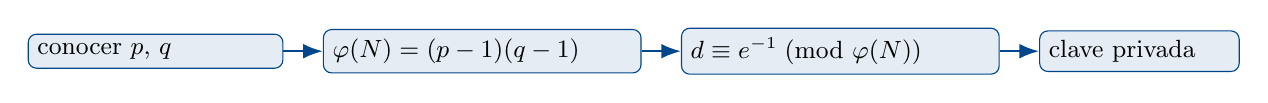
\begin{tikzpicture}[node distance=0.45cm, every node/.style={font=\small}]
    \node[clbox, text width=3cm] (pq)   {conocer $p,\,q$};
    \node[clbox, text width=3.8cm, right=0.5cm of pq]  (phi)
          {$\varphi(N)=(p-1)(q-1)$};
    \node[clbox, text width=3.8cm, right=0.5cm of phi] (d)
          {$d\equiv e^{-1}\!\pmod{\varphi(N)}$};
    \node[clbox, text width=2.3cm, right=0.5cm of d]  (priv)
          {clave privada};
    \draw[flecha, clasico] (pq) -- (phi);
    \draw[flecha, clasico] (phi) -- (d);
    \draw[flecha, clasico] (d) -- (priv);
  \end{tikzpicture}}
  \end{center}

  \begin{itemize}
    \item El atacante conoce $(N,e)$ (públicos).
    \item Si logra \textbf{factorizar $N=p\cdot q$}, calcula $\varphi(N)$
          trivialmente.
    \item Con $\varphi(N)$ y $e$, obtiene $d$ con el
          \textbf{algoritmo de Euclides extendido} (eficiente).
    \item Con $d$ descifra cualquier mensaje y firma como el dueño de la clave.
  \end{itemize}

  \begin{alertblock}{}
    La seguridad de RSA se apoya por completo en que nadie pueda
    factorizar $N$. Shor ataca ese único punto.
  \end{alertblock}

  \note{
    Recalcar: no hace falta ``romper la matemática de RSA''. Basta con
    factorizar. Toda la fortaleza está concentrada en ese cuello de botella.\\[4pt]
    Conectar: el resto de la charla es, en el fondo, ``cómo Shor factoriza $N$''.\\[6pt]
    \textbf{P:} ¿No se puede obtener $\varphi(N)$ sin factorizar?\\
    \textbf{R:} Calcular $\varphi(N)$ para $N=p\cdot q$ es computacionalmente
    equivalente a factorizar; no se conoce atajo.
  }
\end{frame}

%% ── SECCIÓN 2: El problema y prerrequisitos ────────────────────────────────
\section{El problema y prerrequisitos}

%% ── Slide 6: El problema real ─────────────────────────────────────────────
\begin{frame}{El problema real: factorización $\equiv$ order-finding}
  Shor \textbf{no} factoriza por fuerza bruta. Reduce la factorización a:\\[4pt]
  \begin{center}
    \textbf{hallar el período (orden) de una función.}
  \end{center}

  \begin{block}{Definición}
    \small
    Dado $N$ y un $k$ coprimo con $N$, se define $f(x) = k^x \bmod N$.
    Esta función es \textbf{periódica}: existe mínimo $r>0$ tal que
    $f(x+r)=f(x)\;\forall x$, es decir
    $k^r \equiv 1 \pmod{N}$.
    A $r$ se lo llama el \textbf{orden de $k$ módulo $N$}.
  \end{block}

  \begin{exampleblock}{Idea central}
    \small
    Conocer $r$ permite, con álgebra elemental + GCD, recuperar factores de $N$.\\
    Hallar $r$ es \textbf{lo único que necesita la computadora cuántica}.
  \end{exampleblock}

  \note{
    Insistir: el ``milagro'' cuántico no es factorizar directamente, es
    \textbf{encontrar el período}. Todo lo demás es clásico y barato.\\[4pt]
    Intuición de por qué $f$ es periódica: las potencias de $k$ módulo $N$
    viven en un conjunto finito (el grupo multiplicativo $\mathbb{Z}_N^*$), así
    que tarde o temprano se repiten de forma cíclica.\\[6pt]
    \textbf{P:} ¿Por qué $k$ debe ser coprimo con $N$?\\
    \textbf{R:} Si $\gcd(k,N)\neq 1$, ese GCD ya \emph{es} un factor de $N$
    (terminamos sin cuántica). El caso interesante es $\gcd(k,N)=1$, donde
    $f$ es periódica en el grupo multiplicativo.
  }
\end{frame}

%% ── Slide 7: Prerrequisitos sobre N ───────────────────────────────────────
\begin{frame}{Prerrequisitos sobre el input $N$}
  Antes de correr Shor, se descartan clásicamente los casos triviales.
  \textbf{$N$ debe cumplir:}

  \begin{enumerate}
    \item \textbf{$N$ no es primo.}\\
          Si fuera primo, no hay nada que factorizar\\
          (test de primalidad clásico y eficiente, p.\,ej.\ Miller-Rabin).
    \item \textbf{$N$ no es par.}\\
          Si lo fuera, $2$ ya es un factor (se chequea mirando el último bit).
    \item \textbf{$N$ no es una potencia perfecta $n^x$} (con $n,x\in\mathbb{Z}$,
          $x\geq 2$).\\
          Si lo fuera, la raíz $n$ es un factor, hallable con métodos clásicos
          eficientes (probar raíces $x$-ésimas para $x$ hasta $\log_2 N$).
  \end{enumerate}

  Si $N$ pasa estos filtros, es un \textbf{compuesto impar con al menos dos
  factores primos distintos} — el caso para el que Shor está diseñado.

  \note{
    Explicar el porqué de cada descarte: garantizan que existe una
    factorización no trivial y que el método del orden va a funcionar
    (necesitamos $\geq 2$ primos distintos; eso reaparece en la cota de
    probabilidad).\\[4pt]
    Subrayar: estos chequeos son \textbf{clásicos y rápidos}; no
    ``gastamos'' la computadora cuántica en ellos.\\[6pt]
    \textbf{P:} ¿Por qué excluir potencias perfectas si igual son compuestas?\\
    \textbf{R:} Si $N=p^k$ tiene un solo primo, la cota de probabilidad se
    debilita y la raíz se halla trivialmente en clásico. Es más barato
    sacarlas antes.
  }
\end{frame}

%% ── Slide 8: El corazón del algoritmo ────────────────────────────────────
\begin{frame}{El corazón: el período de $f(x)=k^x \bmod N$}
  \begin{itemize}
    \setlength\itemsep{0.25em}
    \item $f(x) = k^x \bmod N$ es \textbf{periódica} con período $r$ = orden
          de $k$ módulo $N$.
    \item Hallar $r$ es \textbf{el único paso que requiere la computadora cuántica}.
    \item Clásicamente no hay método eficiente: el período puede ser
          astronómicamente grande para $N$ de miles de bits.
    \item La cuántica evalúa $f$ en \textbf{superposición sobre todos los $x$}
          y usa interferencia (QFT) para extraer la periodicidad.
  \end{itemize}

  \begin{alertblock}{}
    \small Todos los demás pasos (GCD, chequeos, derivar factores) son
    \textbf{clásicos y polinómicos}. La ventaja cuántica vive enteramente acá.
  \end{alertblock}

  \note{
    Este es el mensaje que debe quedar grabado: \textbf{``lo único cuántico
    es hallar el período''}.\\[4pt]
    Adelantar el mecanismo sin entrar todavía: superposición para evaluar
    todo a la vez + QFT para que la periodicidad se vuelva medible.\\[6pt]
    \textbf{P:} Si la cuántica evalúa todo en paralelo, ¿por qué no leo
    directamente la respuesta?\\
    \textbf{R:} Al medir colapsa a un solo valor al azar. El truco no es el
    paralelismo bruto, sino usar \emph{interferencia} para que lo que se
    mida codifique el período. Lo vemos en la parte de QFT.
  }
\end{frame}

%% ── Slide 9: Esqueleto clásico vs. cuántico (diagrama TikZ) ───────────────
\begin{frame}{Esqueleto del algoritmo: clásico vs.\ cuántico}
  \begin{center}
  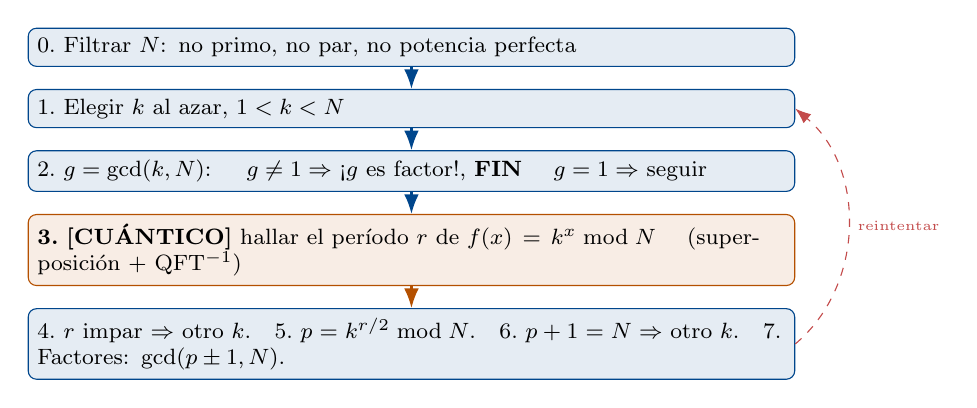
\begin{tikzpicture}[node distance=0.28cm,
    clbox/.style={rectangle, draw=clasico, fill=clasico!10, rounded corners=3pt,
                  text width=9.5cm, align=left, font=\footnotesize},
    qubox/.style={rectangle, draw=cuantico, fill=cuantico!10, rounded corners=3pt,
                  text width=9.5cm, align=left, font=\footnotesize}]
    \node[clbox] (filtro)  {0.\ Filtrar $N$: no primo, no par, no potencia perfecta};
    \node[clbox, below=of filtro] (gcd0)
      {1.\ Elegir $k$ al azar, $1<k<N$};
    \node[clbox, below=of gcd0] (gcd1)
      {2.\ $g=\gcd(k,N)$: \quad
       $g\neq 1\Rightarrow$ ¡$g$ es factor!, \textbf{FIN} \quad
       $g=1\Rightarrow$ seguir};
    \node[qubox, below=of gcd1] (periodo)
      {\textbf{3.\ [CUÁNTICO]} hallar el período $r$ de
       $f(x)=k^x\bmod N$ \quad(superposición + QFT$^{-1}$)};
    \node[clbox, below=of periodo] (post)
      {4.\ $r$ impar $\Rightarrow$ otro $k$.\quad
       5.\ $p=k^{r/2}\bmod N$.\quad
       6.\ $p+1=N\Rightarrow$ otro $k$.\quad
       7.\ Factores: $\gcd(p\pm1,N)$.};
    \draw[flecha, clasico]  (filtro)  -- (gcd0);
    \draw[flecha, clasico]  (gcd0)    -- (gcd1);
    \draw[flecha, clasico]  (gcd1)    -- (periodo);
    \draw[flecha, cuantico] (periodo) -- (post);
    \draw[retry] (post.east) to[bend right=50]
      node[right, font=\tiny\color{alerta}] {reintentar} (gcd0.east);
  \end{tikzpicture}
  \end{center}
  \note{
    Caminar el diagrama de arriba hacia abajo. Señalar visualmente que
    \textbf{un solo bloque es cuántico} (paso 3).\\[4pt]
    Marcar los dos puntos de reintento (pasos 4 y 6): de ahí sale que
    Shor es \textbf{probabilístico}.\\[4pt]
    El paso 2 es un ``regalo'': a veces el $k$ aleatorio ya comparte
    factor con $N$ y terminamos sin cuántica (raro pero gratis).\\[6pt]
    \textbf{P:} ¿Cuántas veces hay que reintentar?\\
    \textbf{R:} Pocas: la probabilidad de éxito por intento es $\geq 1/2$.
  }
\end{frame}

%% ── Slide 10: La parte clásica en detalle ─────────────────────────────────
\begin{frame}{La parte clásica, en detalle}
  \begin{enumerate}
    \item \textbf{Elegir} $k$ uniformemente al azar en $1<k<N$.
    \item \textbf{GCD inicial:} $g=\gcd(k,N)$.
      \begin{itemize}
        \item Si $g\neq 1$: $g$ es factor no trivial $\to$ listo (sin cuántica).
        \item Si $g=1$: $k$ es coprimo con $N$ $\to$ buscar su orden.
      \end{itemize}
    \item \textit{(cuántico: obtener $r$)}
    \item \textbf{Paridad:} si $r$ es impar $\to$ no sirve, elegir otro $k$.
    \item \textbf{Calcular} $p = k^{r/2}\bmod N$.\\
          \textcolor{clasico!70}{\small(por exponenciación binaria: rápido en clásico)}
    \item \textbf{Chequeo de fallo:} si $p = N-1$ (equivale a $k^{r/2}\equiv -1$)
          $\to$ no sirve, otro $k$.
    \item \textbf{Extraer factores:} $\gcd(p-1,N)$ y $\gcd(p+1,N)$ dan
          factores no triviales.
  \end{enumerate}

  \begin{block}{}
    \small\textbf{Nota de notación:} en lo que sigue,
    $p=k^{r/2}\bmod N$ es un \textbf{residuo}, \emph{no} un primo.
    No confundir con los primos $p,q$ de RSA.
  \end{block}

  \note{
    Remarcar que la exponenciación modular del paso 5 se hace por
    square-and-multiply: rapidísima en clásico.\\[4pt]
    Insistir en la convención: $p$ = residuo, no primo. Es la fuente de
    confusión más frecuente en esta charla.\\[6pt]
    \textbf{P:} ¿El GCD final puede dar 1 o $N$ (trivial)?\\
    \textbf{R:} Sí, y por eso existen los chequeos de los pasos 4 y 6:
    descartan de antemano los $k$ que llevarían a GCD trivial.
  }
\end{frame}

%% ── Slide 11: GCD y Euclides ──────────────────────────────────────────────
\begin{frame}[fragile]{GCD y Euclides: honestidad sobre su uso}
  \textbf{¿Cómo se calcula $\gcd(a,N)$?} Con el \textbf{algoritmo de Euclides}:
  \[
    \gcd(a,b):\quad
    \text{mientras } b\neq 0:\; a,b \leftarrow b,\; a\bmod b;\quad
    \text{devolver } a.
  \]
  Idea: $\gcd(a,b)=\gcd(b,\,a\bmod b)$, reduciendo hasta que un término sea 0.

  \begin{columns}[T]
    \column{0.48\textwidth}
    \begin{exampleblock}{¿Se usa en la práctica?}
      \textbf{Sí.} Euclides es eficiente
      ($O((\log N)^2)$ o mejor) y es exactamente lo que se ejecuta para los
      GCDs al implementar Shor en, por ejemplo, Qiskit.
    \end{exampleblock}

    \column{0.48\textwidth}
    \begin{alertblock}{¿Qué \emph{no} se hace clásicamente?}
      El paso de \textbf{hallar el período $r$}: no existe método clásico
      eficiente conocido. Por eso va a la computadora cuántica.
    \end{alertblock}
  \end{columns}

  \vspace{0.4em}
  \begin{block}{}
    \small Los GCDs y el resto del post-procesamiento son baratos.
    La dificultad está concentrada, otra vez, en \textbf{hallar el período}.
  \end{block}

  \note{
    Responder de frente: Euclides no es ``de juguete'', es producción. La
    frontera clásico/cuántico \textbf{no} pasa por el GCD, pasa por el período.\\[4pt]
    Curiosidad: Euclides extendido también es lo que usa RSA para calcular
    $d$ — la misma herramienta aparece a ambos lados.\\[6pt]
    \textbf{P:} ¿Cuán rápido es Euclides?\\
    \textbf{R:} Polinómico en la cantidad de dígitos; el número de pasos
    está acotado por algo proporcional a $\log$ del menor de los dos números
    (relacionado con Fibonacci). Despreciable frente a todo lo demás.
  }
\end{frame}

%% ── SECCIÓN 3: Por qué el período permite factorizar ───────────────────────
\section{Por qué el período permite factorizar}

%% ── Slide 12: El punto de partida ────────────────────────────────────────
\begin{frame}{Por qué el período permite factorizar (1/5): punto de partida}
  Partimos de la definición de $r$:
  \[
    k^r \equiv 1 \pmod{N}
    \;\Longleftrightarrow\;
    k^r - 1 \equiv 0 \pmod{N}
    \;\Longleftrightarrow\;
    N \mid (k^r - 1).
  \]
  Es decir: \textbf{$N$ divide a $k^r-1$.}

  \vspace{0.5em}
  A partir de ahí vamos a demostrar, encadenadas, cuatro cosas:
  \begin{itemize}
    \item[(a)] por qué $r$ debe ser \textbf{par},
    \item[(b)] por qué exigimos $k^{r/2}+1\not\equiv 0\pmod{N}$,
    \item[(c)] por qué $\gcd(k^{r/2}\pm1,N)$ da \textbf{factores no triviales},
    \item[(d)] por qué todo esto ocurre con \textbf{alta probabilidad}.
  \end{itemize}

  \note{
    Dejar claro que esto \textbf{no} es una colección de hechos sueltos:
    es una sola deducción que arranca en $N\mid(k^r-1)$.\\[4pt]
    Pedir a la audiencia que retenga esa única ecuación; todo lo que sigue
    se desprende de ella.\\[6pt]
    \textbf{P:} ¿Por qué $r$ es el período \emph{mínimo} y no cualquier
    exponente con $k^x\equiv 1$?\\
    \textbf{R:} Por definición de orden: $r$ es el menor positivo con
    $k^r\equiv 1$. Esa minimalidad se usa en (b).
  }
\end{frame}

%% ── Slide 13: (a) r debe ser par ─────────────────────────────────────────
\begin{frame}{(a) Por qué $r$ debe ser par}
  Tenemos $N\mid(k^r-1)$. Si $r$ es \textbf{par}, definimos $p_0=r/2$ entero
  y factorizamos como diferencia de cuadrados:
  \[
    k^r - 1
    = \bigl(k^{r/2}\bigr)^2 - 1
    = \underbrace{\bigl(k^{r/2}-1\bigr)}_{\text{factor A}}
      \underbrace{\bigl(k^{r/2}+1\bigr)}_{\text{factor B}}.
  \]
  Esta factorización \textbf{abre la puerta}: $N$ divide al producto de dos
  números más manejables.

  \vspace{0.3em}
  Si $r$ es \textbf{impar}:
  \begin{itemize}
    \item $r/2$ no es entero $\Rightarrow$ esa factorización no existe en $\mathbb{Z}$.
    \item \textbf{Se descarta este $k$ y se reintenta} con otro.
  \end{itemize}

  \begin{block}{}
    \small \textbf{Notación:} definimos $p = k^{r/2}\bmod N$ (el \emph{residuo}).
    Este $p$ \textbf{no} es un primo.
  \end{block}

  \note{
    El truco es la identidad de secundaria $a^2-b^2=(a-b)(a+b)$ con
    $a=k^{r/2}$, $b=1$.\\[4pt]
    Definir acá la notación que se usará en el ejemplo:
    $p=k^{r/2}\bmod N$ (residuo, no primo).\\[6pt]
    \textbf{P:} ¿Qué tan seguido $r$ sale impar?\\
    \textbf{R:} Para $N=15$, todos los $k$ coprimos tienen $r\in\{2,4\}$
    (pares), así que ninguno falla por imparidad.
  }
\end{frame}

%% ── Slide 14: (b) la condición ≢ −1 ────────────────────────────────────
\begin{frame}{(b) Por qué se exige $k^{r/2}+1\not\equiv 0\pmod{N}$}
  De (a): $N\mid\bigl(k^{r/2}-1\bigr)\bigl(k^{r/2}+1\bigr)$.

  Para que esto sea \textbf{útil}, $N$ tiene que \textbf{repartir} sus primos
  entre los dos factores. El intento \textbf{falla} si $N$ divide
  enteramente a uno solo:

  \vspace{0.3em}
  \begin{columns}[T]
    \column{0.48\textwidth}
    \begin{exampleblock}{Subcaso 1 — imposible}
      $N\mid(k^{r/2}-1)$ implica $k^{r/2}\equiv 1\pmod{N}$.\\
      Pero eso contradiría que $r$ es el período \emph{mínimo}.
      $\Rightarrow$ \textbf{no puede ocurrir}.
    \end{exampleblock}

    \column{0.48\textwidth}
    \begin{alertblock}{Subcaso 2 — modo de fallo}
      $N\mid(k^{r/2}+1)$ implica $k^{r/2}\equiv -1\pmod{N}$,\\
      es decir $p=N-1$.\\
      $\Rightarrow$ \textbf{descartar $k$, reintentar.}\\
      Es el fallo del \emph{caso feo k=14}.
    \end{alertblock}
  \end{columns}

  \vspace{0.3em}
  En ambos fallos, $\gcd(k^{r/2}\pm1,N)$ resultaría trivial (1 o $N$).

  \note{
    Intuición: queremos que cada paréntesis se lleve \emph{parte} de los
    primos de $N$. Si uno se lleva \emph{todos}, el GCD no aísla nada nuevo.\\[4pt]
    El primer subcaso ($\equiv 1$) se elimina solo por minimalidad de $r$;
    el segundo ($\equiv -1$) es el modo de fallo genuino a chequear.\\[4pt]
    Anclar con el ejemplo: $k=14$ da $r=2$, $14^1\bmod 15=14=N-1\Rightarrow$ falla.\\[6pt]
    \textbf{P:} ¿Por qué $\equiv -1$ rompe el método?\\
    \textbf{R:} Porque $k^{r/2}+1\equiv 0$, $N$ divide por completo a ese
    factor, y $\gcd(k^{r/2}-1,N)$ se vuelve trivial.
  }
\end{frame}

%% ── Slide 15: (c) por qué GCD da factores ────────────────────────────────
\begin{frame}{(c) Por qué $\gcd(k^{r/2}\pm1,N)$ da factores no triviales}
  Tras el chequeo (b): $N$ \textbf{no} divide enteramente a ninguno de los
  factores $k^{r/2}-1$, $k^{r/2}+1$. Pero sí divide al \textbf{producto}.

  Como $N=q_1\cdot q_2\cdots$, y ningún paréntesis se lleva todos sus primos:
  algún primo divide a $k^{r/2}-1$ y otro a $k^{r/2}+1$.

  \[
    \gcd\!\bigl(k^{r/2}-1,\,N\bigr)
    \quad\text{y}\quad
    \gcd\!\bigl(k^{r/2}+1,\,N\bigr)
  \]
  devuelven \textbf{divisores propios} de $N$ (ni 1 ni $N$).
  Para $N=15$: \textbf{3 y 5}.

  \begin{block}{}
    \small Es el \textbf{GCD} —no la resta directa— lo que aísla el factor.
    Como Euclides es eficiente, \textbf{este paso es clásico y barato}.
  \end{block}

  \note{
    ¿Por qué GCD y no resta? $k^{r/2}-1$ puede ser enorme y no necesariamente
    un factor de $N$; el GCD con $N$ extrae la \emph{parte común}, que sí
    lo es.\\[4pt]
    Cerrar la cadena: (a) dio la factorización, (b) garantizó que es útil,
    (c) extrae los factores con GCD.\\[6pt]
    \textbf{P:} ¿Siempre los dos GCD dan factores, o a veces solo uno?\\
    \textbf{R:} Tras pasar (b), típicamente ambos dan factores complementarios.
    Si $N=p\cdot q$, un GCD da $p$ y $N/p$ da $q$.
  }
\end{frame}

%% ── Slide 16: (d) la cota de probabilidad ───────────────────────────────
\begin{frame}{(d) ``Alta probabilidad'': la cota cuantitativa}
  \begin{theorem}[Nielsen \& Chuang, Teorema A4.13]
    Sea $N$ compuesto impar con $m$ factores primos distintos. Si $k$ se elige
    uniformemente al azar entre los coprimos con $N$:
    \[
      \Pr\!\bigl[r\text{ par y }k^{r/2}\not\equiv -1\pmod{N}\bigr]
      \;\geq\;
      1 - \frac{1}{2^{m-1}}.
    \]
  \end{theorem}

  \begin{columns}[T]
    \column{0.55\textwidth}
    \begin{itemize}
      \item $m\geq 2$ (tras los filtros) $\Rightarrow$
            \textbf{éxito $\geq 1/2$ por intento}.
      \item Más primos distintos $\Rightarrow$ cota $\to 1$.
      \item Reintentos esperados: $\leq 2$.
    \end{itemize}

    \column{0.42\textwidth}
    \begin{exampleblock}{\small Fuente}
      \small El paper de la cátedra \emph{no} incluye esta cota
      (y tiene una errata).\\
      Se cita Nielsen \& Chuang como fuente estándar.
    \end{exampleblock}
  \end{columns}

  \note{
    Explicar el $2^{m-1}$: la fracción de $k$ ``malos'' se reparte por el
    teorema chino del resto entre los $m$ primos; queda acotada por
    $1/2^{m-1}$.\\[4pt]
    Ser honestos: el paper asignado es divulgativo y no incluye la cota;
    por eso citamos Nielsen \& Chuang.\\[6pt]
    \textbf{P:} ¿Y si tengo mala suerte muchas veces seguidas?\\
    \textbf{R:} La probabilidad de fallar $t$ veces seguidas es $\leq 1/2^t$;
    cae exponencialmente. En la práctica, 1 o 2 intentos.
  }
\end{frame}

%% ── SECCIÓN 4: La parte cuántica — QFT y circuitos ────────────────────────
\section{La parte cuántica: QFT y circuitos}

%% ── Slide 17: Hallar el período (visión general) ─────────────────────────
\begin{frame}{La parte cuántica: hallar el período}
  \textbf{Dos registros:}
  \begin{itemize}
    \setlength\itemsep{0.2em}
    \item \textbf{Conteo} ($t$ qubits, $\ket{0}^{\otimes t}$):
          codifica la fase que revela $r$. Se elige $2^t\geq N^2$.
    \item \textbf{Trabajo} ($n=\lceil\log_2 N\rceil$ qubits, $\ket{1}$):
          almacena $k^x\bmod N$.
  \end{itemize}

  \textbf{Pasos:}
  \begin{enumerate}
    \setlength\itemsep{0.1em}
    \item Hadamards en conteo $\to$ superposición uniforme de todos los $x$.
    \item Exponenciación modular controlada:
          $\ket{x}\ket{1}\to\ket{x}\ket{k^x\bmod N}$.
    \item \textbf{QFT$^{-1}$} sobre el registro de conteo.
    \item Medir conteo $\to$ $c\approx s\cdot 2^t/r$.
    \item \textbf{Fracciones continuas} (clásico) $\to$ $r$.
  \end{enumerate}

  \note{
    Aclarar la elección de $t$: con $2^t\geq N^2$ se garantiza que el
    resultado de la medición permite recuperar $r$ por fracciones continuas
    de manera unívoca.\\[4pt]
    El paso 2 entrelaza los dos registros: la periodicidad de $f$ queda
    ``grabada'' en el estado conjunto.\\[6pt]
    \textbf{P:} ¿Por qué $2^t\geq N^2$ y no $\geq N$?\\
    \textbf{R:} Para que la mejor aproximación racional $s/r$ con denominador
    $<N$ sea única; con menos resolución dos fracciones distintas podrían
    confundirse.
  }
\end{frame}

%% ── Slide 18: La QFT ─────────────────────────────────────────────────────
\begin{frame}{La QFT: qué es}
  La \textbf{Transformada de Fourier Cuántica} sobre $n$ qubits
  ($M=2^n$ estados base) actúa:
  \[
    \mathrm{QFT}\,\ket{j}
    = \frac{1}{\sqrt{M}}\sum_{k=0}^{M-1}
      e^{2\pi i\,jk/M}\,\ket{k}.
  \]
  \begin{itemize}
    \item Mapea $\ket{j}$ a una \textbf{superposición con fases que giran}
          a ``frecuencia'' proporcional a $j$.
    \item Sobre una superposición periódica, las fases \textbf{interfieren
          constructivamente} en los múltiplos de $M/r$ y
          \textbf{destructivamente} en el resto.
    \item Al medir, los valores probables están en $c\approx s\cdot M/r$
          $\to$ de ahí se extrae $r$.
  \end{itemize}

  \begin{block}{Implementación eficiente}
    \small Se construye con \textbf{Hadamards} y \textbf{rotaciones de fase
    controladas} $R_d = \mathrm{diag}(1,\,e^{2\pi i/2^d})$.
    Usa $O(n^2)$ compuertas.
  \end{block}

  \note{
    Metáfora: la QFT ``escucha'' el estado y revela en qué frecuencia se
    repite. La periodicidad de $f$ se traduce en picos en el dominio
    transformado.\\[4pt]
    No hace falta derivar la forma producto compuerta a compuerta; basta
    mostrar que son H + rotaciones controladas y que son $O(n^2)$.\\[6pt]
    \textbf{P:} ¿QFT o QFT inversa en Shor?\\
    \textbf{R:} En el circuito de order-finding se aplica la \textbf{QFT
    inversa} (estimación de fase). La diferencia es solo el signo del
    exponente; el costo es el mismo.
  }
\end{frame}

%% ── Slide 19: QFT vs. DFT/FFT ────────────────────────────────────────────
\begin{frame}{QFT vs.\ DFT/FFT clásica}
  \resizebox{\textwidth}{!}{%
  \begin{tabular}{>{\bfseries}l p{5.2cm} p{5.2cm}}
    \toprule
    & \textbf{DFT/FFT (clásica)} & \textbf{QFT (cuántica)} \\
    \midrule
    Sobre qué actúa
      & Vector de $M$ amplitudes explícitas
      & Amplitudes de $n=\log_2 M$ qubits \\[4pt]
    Costo
      & FFT: $O(M\log M)=O(2^n\!\cdot\! n)$
      & $O(n^2)=O((\log M)^2)$ compuertas \\[4pt]
    Salida
      & Todas las $M$ componentes, \textbf{legibles}
      & Una sola muestra (probabilística) \\[4pt]
    Acceso
      & Lectura completa del espectro
      & No se puede leer todo (medición colapsa) \\
    \bottomrule
  \end{tabular}}

  \begin{alertblock}{La diferencia clave}
    La QFT es \textbf{exponencialmente más rápida} en operaciones\ldots\\
    \ldots pero \textbf{no entrega el espectro completo}: solo permite
    \emph{muestrear} una salida.\\
    El arte de Shor: diseñar el circuito para que \textbf{lo que se
    muestrea codifique el período $r$}.
  \end{alertblock}

  \note{
    Desactivar el malentendido común: ``la QFT calcula la FFT más rápido
    y la leo entera''. Falso. No hay lectura completa.\\[4pt]
    La ganancia exponencial se ``paga'' con acceso restringido; por eso
    hace falta el post-procesamiento (fracciones continuas) y la repetición.\\[6pt]
    \textbf{P:} ¿La QFT no sirve para acelerar FFTs comunes?\\
    \textbf{R:} No directamente, porque no se pueden leer todas las salidas.
    Sirve dentro de algoritmos (como Shor) donde alcanza con muestrear
    cierta información estructural.
  }
\end{frame}

%% ── Slide 20: Estimación de fase ─────────────────────────────────────────
\begin{frame}{Estimación de fase: el motor del order-finding}
  El subprograma de período es una \textbf{estimación de fase} del operador $U$:
  \[
    U\ket{y} = \ket{k\cdot y \bmod N}.
  \]
  \begin{itemize}
    \item Los autovectores de $U$ tienen autovalores $e^{2\pi i\,s/r}$
          ($s=0,\ldots,r-1$).
    \item El estado inicial $\ket{1}$ del registro de trabajo es
          \textbf{superposición de esos autovectores}.
    \item Aplicando $U$ controlada $2^j$ veces desde cada qubit de conteo,
          se ``imprime'' la fase $s/r$ en el registro de conteo.
    \item La \textbf{QFT inversa} convierte esa fase en un entero medible
          $c\approx s\cdot 2^t/r$.
  \end{itemize}

  \begin{block}{}
    \small
    $k^x\bmod N$ \;$\longrightarrow$\; periodicidad $r$
    \;$\longrightarrow$\; fases $s/r$
    \;$\longrightarrow$\; $\mathrm{QFT}^{-1}$
    \;$\longrightarrow$\; medir $c\approx s\cdot 2^t/r$.
  \end{block}

  \note{
    Para quien vio estimación de fase: decir explícitamente ``order-finding
    = estimación de fase de la compuerta de multiplicación por $k$''.\\[4pt]
    Para quien no: la idea operativa es que las potencias controladas de
    $U$ graban la fase $s/r$ en el registro de conteo, y la QFT$^{-1}$ la
    vuelve legible como entero.\\[6pt]
    \textbf{P:} ¿Por qué arrancar el registro de trabajo en $\ket{1}$ y no
    en $\ket{0}$?\\
    \textbf{R:} $\ket{1}$ es combinación de todos los autovectores relevantes
    de $U$, lo que permite que cualquier $s$ aparezca. $\ket{0}$ sería
    absorbido ($0\cdot k=0$) y no daría información.
  }
\end{frame}

%% ── Slide 21: El circuito cuántico completo (quantikz) ───────────────────
\begin{frame}{El circuito cuántico completo}
  \[
  \resizebox{0.9\textwidth}{!}{%
  \begin{quantikz}[row sep=0.25cm]
    \lstick{$\ket{0}$} & \gate{H} & \ctrl{3} & \qw      & \gate[3]{\mathrm{QFT}^{-1}} & \meter{} \\
    \lstick{\vdots}    &          &          & \ddots   &                              & \vdots   \\
    \lstick{$\ket{0}$} & \gate{H} & \qw      & \ctrl{1} &                              & \meter{} \\
    \lstick{$\ket{1}^{\otimes n}$} \qwbundle{n} & \qw & \gate{U^{2^0}} & \gate{U^{2^{t-1}}} & \qw & \qw
  \end{quantikz}}
  \]

  \vspace{0.15em}
  {\small
  \textbf{1.} $H$ $\to$ superposición. \quad
  \textbf{2.} Exp.\ modular controlada: $\ket{x}\ket{1}\to\ket{x}\ket{k^x\bmod N}$. \quad
  \textbf{3.} QFT$^{-1}$. \quad
  \textbf{4.} Medir conteo $\to c$. (Trabajo: no se mide.)
  }

  \note{
    Recorrer las cuatro capas. Enfatizar que las mediciones son solo del
    registro de conteo.\\[4pt]
    El registro de trabajo ``se sacrifica'': su rol es entrelazarse para
    grabar la fase; no se lee.\\[6pt]
    \textbf{P:} ¿Cuántos qubits en total?\\
    \textbf{R:} $t+n$, con $t\approx 2\log_2 N$ y $n\approx\log_2 N$. Para
    $N=15$: $t=8$, $n=4$ $\to$ 12 qubits (las implementaciones optimizadas
    usan muchos menos).
  }
\end{frame}

%% ── Slide 22: El bloque costoso (U) ─────────────────────────────────────
\begin{frame}{El bloque costoso: exponenciación modular controlada}
  \[
    U:\ket{y}\to\ket{k\cdot y\bmod N}
    \qquad\text{encadenando:}\qquad
    \ket{x}\ket{1}\to\ket{x}\ket{k^x\bmod N}
  \]

  \begin{itemize}
    \item Se trata como un \textbf{bloque abstracto} en el circuito
          (no desarrollamos su construcción interna a nivel compuertas).
    \item Internamente: sumadores modulares, multiplicadores y exponenciación
          por cuadrados controlada.
    \item \textbf{Es el bloque más costoso del algoritmo:} domina el conteo
          de compuertas y de qubits auxiliares (ancillas). La complejidad total
          de Shor está gobernada por este paso.
  \end{itemize}

  \begin{block}{}
    \small En implementaciones reales (Qiskit y similares) esta es la parte
    que más recursos consume y la más optimizada. La QFT, en comparación,
    es barata.
  \end{block}

  \note{
    Justificar la decisión de mostrarlo como caja: su construcción interna
    es un tema en sí mismo. Lo importante: \textbf{acá está el cuello de
    botella de recursos}.\\[4pt]
    Conectar con complejidad: el $O((\log N)^3)$ viene esencialmente de
    este bloque.\\[6pt]
    \textbf{P:} ¿Por qué es reversible si exponenciar ``pierde'' información?\\
    \textbf{R:} Se implementa conservando el input: $\ket{x}\ket{0}\to
    \ket{x}\ket{k^x\bmod N}$. Toda compuerta cuántica es unitaria, así que
    se diseña para no descartar información (usando ancillas y
    des-computación).
  }
\end{frame}

%% ── Slide 23: Fracciones continuas ───────────────────────────────────────
\begin{frame}{De la medición al período: fracciones continuas}
  La medición da $c$ con $c/2^t\approx s/r$ (para algún $s$ desconocido).
  Para recuperar $r$ se usa el \textbf{desarrollo en fracciones continuas}
  de $c/2^t$: sus \textbf{convergentes} dan la mejor aproximación racional
  con denominador acotado, y ese denominador es (un divisor de) $r$.

  \[
    \frac{c}{2^t} = a_0 + \cfrac{1}{a_1+\cfrac{1}{a_2+\cdots}}
    \;\longrightarrow\;
    \text{convergentes } \frac{p_i}{q_i}
    \;\longrightarrow\;
    r = q_i.
  \]

  \begin{exampleblock}{Importante para $N=15$}
    \small Todos los $k$ coprimos tienen $r\in\{2,4\}$ (potencias de 2).
    Las fracciones $s/r$ salen \textbf{exactas} y las fracciones continuas son
    triviales. \textbf{No hay ``caso feo'' de fracciones continuas con $N=15$.}
    Un caso no trivial requeriría $N$ mayor (p.\,ej.\ $N=21$, $r=6$).
  \end{exampleblock}

  \note{
    Dejar clarísima la aclaración del brief: el único ``caso feo'' con 15
    es el \textbf{fallo por $p=N-1$} ($k=14$), \textbf{no} un
    post-procesamiento complicado de fracciones continuas.\\[4pt]
    Si preguntan por el caso no trivial: $N=21$ con $r=6$ obliga a usar
    convergentes en serio, pero no está en el alcance.\\[6pt]
    \textbf{P:} ¿Por qué fracciones continuas y no redondear?\\
    \textbf{R:} Porque $r$ es lo desconocido. Las fracciones continuas
    recuperan el denominador $r$ a partir solo de $c/2^t$, sin conocerlo
    de antemano.
  }
\end{frame}

%% ── SECCIÓN 5: Ejemplo resuelto N = 15 ────────────────────────────────────
\section{Ejemplo resuelto: $N=15$}

%% ── Slide 24: Preparación ────────────────────────────────────────────────
\begin{frame}{Ejemplo $N=15$: preparación}
  \textbf{Filtros (prerrequisitos):}
  \begin{itemize}
    \item ¿Primo? No ($15=3\times5$). \quad
          ¿Par? No. \quad
          ¿Potencia perfecta? No.
    \item[$\checkmark$] 15 es compuesto impar con 2 primos distintos.
          \textbf{Apto para Shor.}
  \end{itemize}

  \textbf{Registros:}
  $n=\lceil\log_2 15\rceil=4$ qubits (trabajo); \;
  $2^t\geq 225\Rightarrow t=8$ qubits ($2^8=256$).

  \begin{alertblock}{\textbf{Notación importante}}
    \small $p = k^{r/2}\bmod 15$ es un \textbf{residuo},
    \emph{no} un primo. Los factores buscados son 3 y 5.
  \end{alertblock}

  Dos casos:
  \textcolor{alerta}{\textbf{Caso feo (fallo): $k=14$.}} \quad
  \textcolor{cuantico!80!black}{\textbf{Caso feliz (éxito): $k=7$.}}

  \note{
    Mostrar que los filtros son instantáneos.\\[4pt]
    Reforzar la advertencia de notación: $p$ = residuo, no primo. Es la
    fuente de confusión más frecuente en esta charla.\\[6pt]
    \textbf{P:} ¿No es trampa que ya sepamos que $15=3\times5$?\\
    \textbf{R:} Sí, 15 es didáctico. El punto es ver el mecanismo completo
    funcionando con números chequeables a mano.
  }
\end{frame}

%% ── Slide 25: Caso feo k=14 ──────────────────────────────────────────────
\begin{frame}{Caso feo (fallo): $k=14$}
  \begin{block}{1. Coprimalidad}
    $\gcd(14,15)=1$ \checkmark \quad(coprimo, seguimos)
  \end{block}

  \begin{block}{2. Período $f(x)=14^x\bmod 15$}
    \begin{tabular}{c|cccccc}
      $x$       & 0 & 1  & 2 & 3  & 4 & \ldots \\
      $14^x$    & 1 & 14 & 1 & 14 & 1 & \ldots
    \end{tabular}
    \quad$\Rightarrow r=2$ (par \checkmark)
  \end{block}

  \begin{block}{3. Calcular $p=14^{r/2}\bmod 15 = 14^1\bmod 15 = 14$}
  \end{block}

  \begin{alertblock}{4. Chequeo de fallo: $p+1=15=N$ \; \textbf{¡FALLA!}}
    $14^{r/2}\equiv -1\pmod{15}$: $N$ divide por completo a $(p+1)$.\\[2pt]
    Si igual calculáramos:
    \;$\gcd(13,15)=1$ \quad $\gcd(15,15)=15$ \quad $\to$ \textbf{triviales.}\\[2pt]
    \textbf{Conclusión:} $k=14$ no factoriza. Reintentar con otro $k$.
  \end{alertblock}

  \note{
    Este caso ilustra el modo de fallo (b)-$\equiv-1$ con números a la vista.
    $r$ era par (no falló por imparidad) y aun así no sirvió.\\[4pt]
    Shor es \textbf{probabilístico}: hay dos modos de fallo — $r$ impar, o
    $k^{r/2}\equiv -1$. Acá vimos el segundo.\\[6pt]
    \textbf{P:} ¿$k=14$ no es simplemente $-1\bmod 15$?\\
    \textbf{R:} Exacto: $14\equiv -1\pmod{15}$, así que $14^2\equiv 1$ y
    su orden es 2, con $14^1\equiv -1$. El ejemplo más limpio del modo de
    fallo.
  }
\end{frame}

%% ── Slide 26: Caso feliz k=7 — parte clásica ─────────────────────────────
\begin{frame}{Caso feliz ($k=7$): parte clásica}
  \begin{block}{1. $\gcd(7,15)=1$ \checkmark}
  \end{block}

  \begin{block}{2. Período $f(x)=7^x\bmod 15$ \quad (lo calculamos en la cuántica)}
    \begin{tabular}{c|cccccccc}
      $x$    & 0 & 1 & 2 & 3  & 4 & 5 & 6 & \ldots \\
      $7^x$  & 1 & 7 & 4 & 13 & 1 & 7 & 4 & \ldots
    \end{tabular}
    \quad$\Rightarrow r=4$ (par \checkmark)
  \end{block}

  \begin{block}{3. $p = 7^{r/2}\bmod 15 = 7^2\bmod 15 = 49\bmod 15 = 4$}
  \end{block}

  \begin{block}{4. Chequeo: $p+1=5\neq 15$ \checkmark \quad ($7^2\not\equiv -1$)}
  \end{block}

  \begin{exampleblock}{5. Extraer factores con GCD}
    \[
      \gcd(p-1,\,15)=\gcd(3,\,15)=\mathbf{3}
      \qquad
      \gcd(p+1,\,15)=\gcd(5,\,15)=\mathbf{5}
    \]
    \centering\textbf{Factores de 15: 3 y 5. \checkmark\checkmark}
  \end{exampleblock}

  \note{
    Mostrar la cadena completa (a)$\to$(b)$\to$(c) instanciada: $r$ par,
    $p\neq N-1$, GCDs dan 3 y 5.\\[4pt]
    Verificar en voz alta: $3\times5=15$. Cierra.\\[6pt]
    \textbf{P:} ¿Y si me hubiera tocado $k=4$ ($r=2$)?\\
    \textbf{R:} $4^1\bmod 15=4$, $p+1=5\neq15$, $\gcd(3,15)=3$,
    $\gcd(5,15)=5$. También funciona.
  }
\end{frame}

%% ── Slide 27: Caso k=7 — periodicidad ────────────────────────────────────
\begin{frame}{Caso $k=7$ — parte cuántica: la periodicidad}
  $f(x)=7^x\bmod 15$, evaluada en superposición:

  \begin{center}
  \begin{tabular}{c|cccccccc}
    \toprule
    $x$     & 0 & 1 & 2 & 3  & 4 & 5 & 6 & \ldots \\
    \midrule
    $7^x\bmod 15$ & 1 & 7 & 4 & 13 & 1 & 7 & 4 & \ldots \\
    \bottomrule
  \end{tabular}
  \end{center}

  \vspace{0.4em}
  La secuencia $1,7,4,13,1,7,4,13,\ldots$ \textbf{se repite cada 4 pasos}
  $\Rightarrow$ período $r=4$.

  El registro de trabajo, tras la exponenciación modular, queda
  \textbf{entrelazado} con el de conteo: para cada $x$, almacena
  $7^x\bmod 15\in\{1,7,4,13\}$.

  \begin{block}{}
    \small Esta periodicidad es la ``señal'' que la QFT$^{-1}$ va a convertir
    en picos en el dominio transformado.
  \end{block}

  \note{
    Mostrar el ciclo de 4 valores explícito.\\[4pt]
    Clásicamente detectar este período para $N$ grande sería inviable;
    acá es chico para verlo a mano.\\[6pt]
    \textbf{P:} ¿El registro de trabajo toma los 4 valores a la vez?\\
    \textbf{R:} Sí, en superposición entrelazada con $x$. No lo medimos:
    medir el registro de conteo (tras QFT$^{-1}$) es lo que revela el período.
  }
\end{frame}

%% ── Slide 28: El circuito concreto k=7, N=15 ─────────────────────────────
\begin{frame}{Caso $k=7$ — el circuito concreto ($t=8$, $n=4$)}
  \[
  \begin{quantikz}[row sep=0.5cm]
    \lstick{$\ket{0}^{\otimes 8}$} \qwbundle{8}
      & \gate{H^{\otimes 8}} & \ctrl{1}
      & \gate{\mathrm{QFT}^{-1}} & \meter{c} \\
    \lstick{$\ket{1}\!=\!\ket{0001}$} \qwbundle{4}
      & \qw & \gate[style={fill=cuantico!10}]{\text{U: }|y\rangle\to|7y\bmod15\rangle}
      & \qw & \qw
  \end{quantikz}
  \]

  \begin{itemize}
    \item \textbf{Conteo:} 8 qubits ($2^8=256\geq 225=15^2$).
    \item \textbf{Trabajo:} 4 qubits, init $\ket{1}=\ket{0001}$.
    \item \textbf{Bloque $U$:} multiplicación por 7 módulo 15, $2^j$ veces
          controlada por el qubit $j$ de conteo (mostrado como caja abstracta).
    \item QFT$^{-1}$ sobre los 8 qubits de conteo, luego medición.
  \end{itemize}

  \note{
    Es el mismo circuito genérico de la slide anterior, ahora con números:
    $k=7$, $N=15$, $t=8$, $n=4$.\\[4pt]
    Esta es la versión ``de libro''; las demostraciones históricas con 15
    usaron circuitos comprimidos con conocimiento previo de la respuesta.\\[6pt]
    \textbf{P:} ¿8 qubits de conteo no es mucho para $N=15$?\\
    \textbf{R:} Para garantizar fracciones continuas unívocas se usa
    $t\approx 2\log_2 N$. Con $r$ potencia de 2 alcanzaría con menos,
    pero mantenemos la regla general.
  }
\end{frame}

%% ── Slide 29: Mediciones y fracciones continuas ──────────────────────────
\begin{frame}{Caso $k=7$ — mediciones y fracciones continuas}
  Con $r=4$ y $2^t=256$, los picos de la QFT$^{-1}$ están en
  $c\approx s\cdot 64$ ($s=0,1,2,3$):

  \resizebox{\textwidth}{!}{%
  \begin{tabular}{ccccl}
    \toprule
    $c$ & $c/256$ & fracción reducida & denominador & resultado \\
    \midrule
    0   & 0       & 0                 & —           & inútil ($s=0$), repetir \\
    64  & 1/4     & \textbf{1/4}      & \textbf{4}  & \textcolor{cuantico!80!black}{$r=4$ \checkmark} \\
    128 & 1/2     & 1/2               & 2           & candidato $r=2$; $7^2\bmod15=4\neq1\to$ repetir \\
    192 & 3/4     & \textbf{3/4}      & \textbf{4}  & \textcolor{cuantico!80!black}{$r=4$ \checkmark} \\
    \bottomrule
  \end{tabular}}

  \vspace{0.2em}
  Con pocas mediciones, se obtiene $r=4$ con altísima probabilidad.

  \note{
    La medición es probabilística: no todos los outcomes sirven, pero la
    mayoría sí, y los inútiles se detectan verificando $k^{\text{candidato}}\bmod N=1$.\\[4pt]
    El caso $c=128\to 1/2$ es pedagógico: el denominador es un divisor de
    $r$ y hay que verificar/repetir.\\[6pt]
    \textbf{P:} ¿Cómo sé que $r=2$ es falso?\\
    \textbf{R:} $7^2\bmod15=4\neq1$, así que 2 no es período. La
    verificación es clásica y barata.\\
    \textbf{P:} ¿Las probabilidades de cada pico son iguales?\\
    \textbf{R:} Para $r\mid 2^t$ (como acá), los cuatro picos son exactos
    y equiprobables ($\approx1/4$ cada uno).
  }
\end{frame}

%% ── Slide 30: Cierre del ejemplo ─────────────────────────────────────────
\begin{frame}{Caso $k=7$ — cierre del ejemplo}
  \begin{center}
  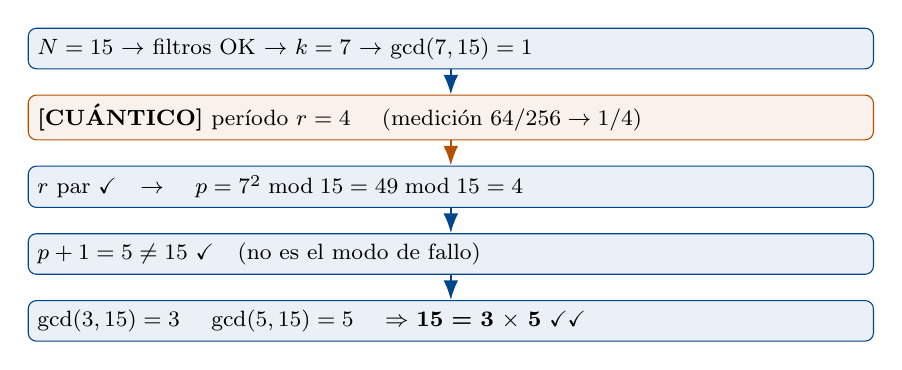
\begin{tikzpicture}[node distance=0.32cm,
    cbox/.style={rectangle, draw=clasico, fill=clasico!8, rounded corners=3pt,
                 text width=10.5cm, align=left, font=\footnotesize},
    qbox/.style={rectangle, draw=cuantico, fill=cuantico!8, rounded corners=3pt,
                 text width=10.5cm, align=left, font=\footnotesize}]
    \node[cbox] (f) {$N=15$ $\to$ filtros OK $\to$ $k=7$ $\to$ $\gcd(7,15)=1$};
    \node[qbox, below=of f] (q)
      {\textbf{[CUÁNTICO]} período $r=4$ \quad(medición $64/256\to 1/4$)};
    \node[cbox, below=of q] (p) {$r$ par \checkmark $\quad\to\quad$ $p=7^2\bmod15=49\bmod15=4$};
    \node[cbox, below=of p] (ch) {$p+1=5\neq15$ \checkmark \quad(no es el modo de fallo)};
    \node[cbox, below=of ch] (g)
      {$\gcd(3,15)=3$ \quad $\gcd(5,15)=5$ \quad $\Rightarrow$ \textbf{15 = 3 $\times$ 5 \checkmark\checkmark}};
    \draw[flecha, clasico]  (f) -- (q);
    \draw[flecha, cuantico] (q) -- (p);
    \draw[flecha, clasico]  (p) -- (ch);
    \draw[flecha, clasico]  (ch)-- (g);
  \end{tikzpicture}
  \end{center}

  \note{
    Cerrar el arco narrativo: un fallo (14) y un éxito (7), mismo $N$,
    todo a mano.\\[4pt]
    Reconectar con la teoría: este ejemplo instanció las cuatro piezas
    (a, b, c, d) de la cadena algebraica.\\[6pt]
    \textbf{P:} En $N$ grande, ¿este mismo procedimiento escala?\\
    \textbf{R:} Sí, idéntico. Lo único que crece es el costo de la parte
    cuántica (más qubits, bloque de exponenciación más grande).
  }
\end{frame}

%% ── Slide 31: Flujo completo (TikZ) ──────────────────────────────────────
\begin{frame}{El flujo completo, de un vistazo}
  \begin{center}
  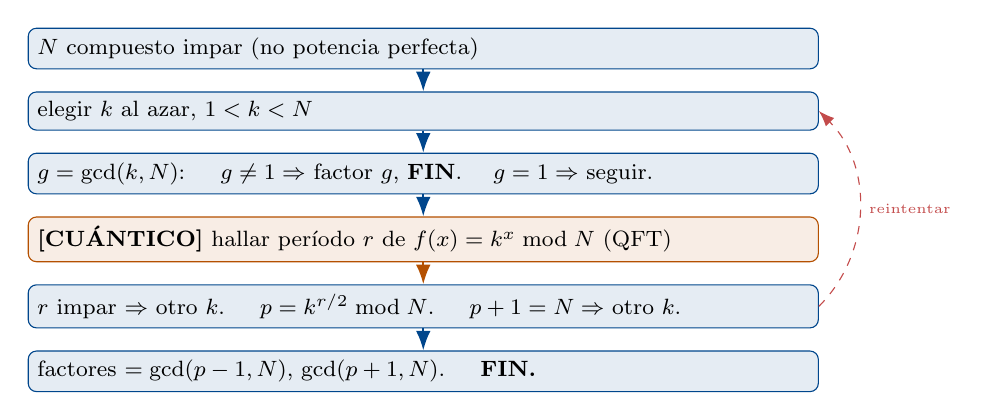
\begin{tikzpicture}[node distance=0.28cm,
    clbox/.style={rectangle, draw=clasico, fill=clasico!10, rounded corners=3pt,
                  text width=9.8cm, align=left, font=\footnotesize},
    qubox/.style={rectangle, draw=cuantico, fill=cuantico!10, rounded corners=3pt,
                  text width=9.8cm, align=left, font=\footnotesize}]
    \node[clbox] (n)  {$N$ compuesto impar (no potencia perfecta)};
    \node[clbox, below=of n] (k)  {elegir $k$ al azar, $1<k<N$};
    \node[clbox, below=of k] (g)
      {$g=\gcd(k,N)$: \quad $g\neq1\Rightarrow$ factor $g$, \textbf{FIN}. \quad $g=1\Rightarrow$ seguir.};
    \node[qubox, below=of g] (r)
      {\textbf{[CUÁNTICO]} hallar período $r$ de $f(x)=k^x\bmod N$ (QFT)};
    \node[clbox, below=of r] (par)
      {$r$ impar $\Rightarrow$ otro $k$. \quad $p=k^{r/2}\bmod N$. \quad
       $p+1=N\Rightarrow$ otro $k$.};
    \node[clbox, below=of par] (fin)
      {factores $=\gcd(p-1,N)$, $\gcd(p+1,N)$. \quad \textbf{FIN.}};
    \draw[flecha, clasico]  (n)   -- (k);
    \draw[flecha, clasico]  (k)   -- (g);
    \draw[flecha, clasico]  (g)   -- (r);
    \draw[flecha, cuantico] (r)   -- (par);
    \draw[flecha, clasico]  (par) -- (fin);
    \draw[retry] (par.east) to[bend right=45]
      node[right, font=\tiny\color{alerta}] {reintentar} (k.east);
  \end{tikzpicture}
  \end{center}
  \note{
    Usar este slide como resumen/repaso antes de pasar a complejidad.\\[4pt]
    Señalar el único bloque cuántico y los dos puntos de reintento.
  }
\end{frame}

%% ── SECCIÓN 6: Complejidad e implicancias ──────────────────────────────────
\section{Complejidad e implicancias}

%% ── Slide 32: Complejidad Shor vs. GNFS ─────────────────────────────────
\begin{frame}{Complejidad: Shor vs.\ el mejor clásico (GNFS)}
  Comparamos \textbf{tiempo} para factorizar un entero de $n=\log_2 N$ bits.

  \begin{columns}[T]
    \column{0.5\textwidth}
    \begin{block}{GNFS (mejor clásico) — sub-exponencial}
      \small
      \[
        \exp\!\Bigl(\bigl(\tfrac{64}{9}\bigr)^{1/3}
          (\ln N)^{1/3}(\ln\!\ln N)^{2/3}\Bigr)
      \]
      Crece más lento que exponencial puro, pero \textbf{mucho} más rápido
      que cualquier polinomio.
    \end{block}

    \column{0.47\textwidth}
    \begin{exampleblock}{Shor (cuántico) — polinómico}
      \small
      \[
        O\!\bigl((\log N)^3\bigr)
      \]
      (versión estándar; $\tilde{O}((\log N)^2)$ con multiplicación rápida)\\[3pt]
      + post-procesamiento clásico polinómico.
    \end{exampleblock}
  \end{columns}

  \begin{alertblock}{}
    \small Salto cualitativo: \textbf{sub-exponencial $\to$ polinómico.}
    No es ``una constante mejor'': es otra clase de complejidad.
  \end{alertblock}

  \note{
    Las cotas finas de Shor vienen de Nielsen \& Chuang / Shor 1994, \textbf{no}
    del paper de la cátedra (que solo dice vagamente ``raíz cuadrada del
    tiempo'', afirmación imprecisa que conviene corregir).\\[4pt]
    El costo está dominado por la exponenciación modular (bloque $U$).\\[6pt]
    \textbf{P:} ¿``Polinómico'' significa rápido en la práctica hoy?\\
    \textbf{R:} Polinómico en operaciones lógicas ideales. En hardware real,
    la corrección de errores multiplica enormemente los recursos físicos.
  }
\end{frame}

%% ── Slide 33: Crecimiento comparativo (TikZ) ────────────────────────────
\begin{frame}{Crecimiento comparativo (intuición)}
  \begin{center}
  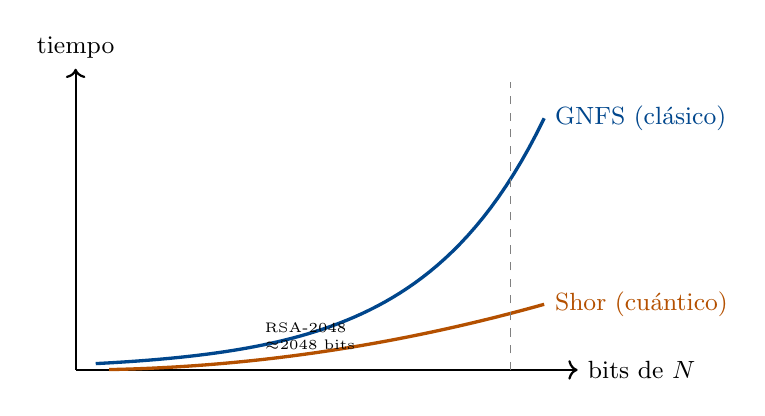
\begin{tikzpicture}[scale=0.85]
    \draw[->,thick] (0,0) -- (7.5,0) node[right]{\small bits de $N$};
    \draw[->,thick] (0,0) -- (0,4.5) node[above]{\small tiempo};

    % GNFS (sub-exponencial) — curva que sube rápido, siempre arriba
    \draw[clasico, very thick, domain=0.3:7, samples=60]
      plot (\x, {0.08*exp(0.55*\x)})
      node[right]{\small\textcolor{clasico}{GNFS (clásico)}};

    % Shor (polinómico) — curva que crece suave, siempre abajo
    \draw[cuantico, very thick, domain=0.5:7, samples=60]
      plot (\x, {0.02*\x^2})
      node[right]{\small\textcolor{cuantico}{Shor (cuántico)}};

    \node[align=left, font=\tiny] at (3.5, 0.5) {RSA-2048\\$\approx$2048 bits};
    \draw[dashed, gray] (6.5,0) -- (6.5,4.3);
  \end{tikzpicture}
  \end{center}
  \small
  Para claves RSA reales (2048+ bits), GNFS se va a tiempos astronómicos;
  Shor se mantiene tratable (en una máquina cuántica ideal suficientemente grande).

  \note{
    Gráfico cualitativo, no a escala. El mensaje es la \textbf{forma} de
    las curvas: una explota, la otra crece suave.\\[4pt]
    Recordar el ``pero'': ``máquina cuántica ideal suficientemente grande''
    es el gran condicional; lo aterrizamos en las próximas slides.
  }
\end{frame}

%% ── Slide 34: Implicancias en la criptografía actual ─────────────────────
\begin{frame}{Implicancias en la criptografía actual}
  \begin{columns}[T]
    \column{0.5\textwidth}
    \begin{alertblock}{Qué \textbf{rompe} Shor}
      \begin{itemize}\small
        \item \textbf{RSA} (factorización) — cifrado y firma.
        \item \textbf{DH, ElGamal, DSA} (log.\,discreto) — variante de Shor.
        \item \textbf{ECDH, ECDSA} (log.\,discreto en curvas) — también caen,
              con menos qubits que RSA.
      \end{itemize}
    \end{alertblock}

    \column{0.47\textwidth}
    \begin{exampleblock}{Qué \textbf{NO} rompe (o debilita levemente)}
      \begin{itemize}\small
        \item \textbf{AES:} el ataque cuántico relevante es \textbf{Grover}
              (cuadrático). Se mitiga duplicando el tamaño de clave.
        \item \textbf{SHA-2/3:} igual, Grover cuadrático $\to$ usar hashes
              más largos.
      \end{itemize}
    \end{exampleblock}
  \end{columns}

  \begin{block}{}
    \small La criptografía de \textbf{clave pública clásica} es la víctima
    principal; la simétrica sobrevive con claves más largas.
  \end{block}

  \note{
    Distinguir claramente: Shor mata la \textbf{clave pública} basada en
    factorización/log discreto; \textbf{no} mata la simétrica.\\[4pt]
    Grover $\neq$ Shor: Grover es búsqueda, aceleración cuadrática, fácil
    de compensar. Es un error común confundirlos.\\[6pt]
    \textbf{P:} ¿AES-256 está bien?\\
    \textbf{R:} Frente a lo conocido hoy, sí: Grover lo lleva a $\sim$128
    bits de seguridad efectiva, todavía robusto.
  }
\end{frame}

%% ── Slide 35: Estado actual del hardware cuántico ────────────────────────
\begin{frame}{Estado actual del hardware cuántico (2025--2026)}
  \begin{itemize}
    \item \textbf{Google ``Willow'' (fines 2024):} 105 qubits superconductores.
          Demostró \textbf{corrección de errores ``por debajo del umbral''}
          (el error lógico baja al agregar qubits físicos). Hito cualitativo,
          no una máquina factorizadora.
    \item \textbf{IBM — hoja de ruta a tolerancia a fallos:}
          sistema \textbf{``Starling'' para 2029} con $\sim$200 qubits lógicos
          y 100M de operaciones corregidas; hitos intermedios \emph{Loon} (2025),
          \emph{Kookaburra} (2026), \emph{Cockatoo} (2027). Meta de
          $\sim$1000 qubits lógicos a inicios de 2030, con códigos qLDPC.
    \item \textbf{Realidad para Shor:} no existe hoy una máquina capaz de
          correr Shor sobre números criptográficamente relevantes. Falta
          tolerancia a fallos a escala.
  \end{itemize}

  \begin{block}{}
    \small \textbf{Qubits físicos} (ruidosos, abundantes)
    vs.\ \textbf{qubits lógicos} (corregidos, escasos).
    Shor a escala RSA necesita miles de lógicos.
  \end{block}

  \note{
    Citar fechas y fuentes. Estos datos envejecen rápido: revisar antes
    de cada exposición.\\[4pt]
    El punto honesto: hay progreso real y sostenido, pero romper RSA sigue
    estando a años de distancia según las hojas de ruta públicas.\\[6pt]
    \textbf{P:} ¿Cuándo se rompe RSA-2048?\\
    \textbf{R:} Nadie lo sabe con certeza. Las hojas de ruta apuntan a la
    década de 2030 para máquinas con miles de qubits lógicos. Por eso la
    migración a PQC empieza \textbf{ahora} (riesgo ``harvest now, decrypt later'').
  }
\end{frame}

%% ── Slide 36: El gap honesto ─────────────────────────────────────────────
\begin{frame}{El ``gap'' honesto: lo más grande factorizado de verdad}
  \begin{columns}[T]
    \column{0.55\textwidth}
    \begin{alertblock}{En hardware cuántico real (Shor genuino)}
      \begin{itemize}\small
        \item \textbf{15} (2001, IBM, $\sim$8 qubits) — récord confiable.
        \item \textbf{21} (2012, $\sim$10 qubits).
        \item Muchos ``récords'' mediáticos usan circuitos
              \textbf{pre-compilados} (con los factores conocidos de antemano)
              o métodos adiabáticos/de optimización que \textbf{no escalan}.
              No cuentan como Shor genuino.
      \end{itemize}
    \end{alertblock}

    \column{0.42\textwidth}
    \begin{exampleblock}{En simulación clásica}
      \small Se han simulado semiprimos de $\sim$12 dígitos, pero eso
      mide la simulación, no una ventaja cuántica real.
    \end{exampleblock}

    \begin{block}{}
      \small La distancia entre ``15 en hardware'' y ``2048 bits en RSA''
      es \textbf{enorme}. La amenaza es futura y creíble, no presente.
    \end{block}
  \end{columns}

  \note{
    Este slide es el antídoto contra el hype. Si la audiencia se queda con
    una sola idea escéptica, que sea esta.\\[4pt]
    ¿Por qué los ``récords grandes'' son engañosos? Si ya se conocen los
    factores, se comprime el circuito a algo trivial; no demuestra capacidad
    de factorizar lo desconocido.\\[6pt]
    \textbf{P:} ¿Y los titulares de factorizar números enormes?\\
    \textbf{R:} Casi siempre son recocido cuántico (D-Wave) o trucos de
    compilación, no Shor escalable.
  }
\end{frame}

%% ── Slide 37: Estimaciones de recursos ───────────────────────────────────
\begin{frame}{Estimaciones de recursos para romper RSA-2048}
  \begin{columns}[T]
    \column{0.55\textwidth}
    \begin{block}{Gidney \& Ekerå (2019)}
      \small $\sim$\textbf{20 millones} de qubits físicos ruidosos, $\sim$8 horas.
    \end{block}

    \begin{exampleblock}{Gidney (mayo 2025, arXiv:2505.15917)}
      \small \textbf{Menos de 1 millón} de qubits físicos, \textbf{$<$1 semana}.\\
      ($\approx$\textbf{1399 qubits lógicos})\\[2pt]
      Reducción de $\sim$20$\times$ respecto de 2019, por mejor aritmética
      modular y codificación más eficiente.
    \end{exampleblock}

    \column{0.42\textwidth}
    \begin{alertblock}{Lectura}
      \small
      \begin{itemize}
        \item La barrera \textbf{sigue siendo enorme} frente a las máquinas
              actuales.
        \item Las estimaciones \textbf{bajan año a año}: el blanco se acerca
              por mejoras de algoritmo y de corrección.
        \item No hace falta esperar la máquina para preocuparse.
      \end{itemize}
    \end{alertblock}
  \end{columns}

  \note{
    Contar la historia 2019$\to$2025: cada avance algorítmico recorta
    requisitos.\\[4pt]
    Las reducciones son en el \emph{modelo de recursos}; construir $\sim$1M
    de qubits físicos con corrección sigue siendo un desafío de ingeniería
    de años. Pero justifica migrar ya.\\[6pt]
    \textbf{P:} Si baja tan rápido, ¿no será inminente?\\
    \textbf{R:} Las reducciones son en el modelo de recursos ideales.
    Construir la máquina física sigue siendo un desafío de años. Pero
    justifica migrar ahora.
  }
\end{frame}

%% ── Slide 38: NIST PQC ───────────────────────────────────────────────────
\begin{frame}{Criptografía post-cuántica: NIST PQC}
  Algoritmos diseñados para resistir a Shor y Grover, corribles en hardware
  clásico. \textbf{NIST} finalizó los primeros estándares:

  \begin{center}
  {\small
  \begin{tabular}{llll}
    \toprule
    \textbf{Estándar} & \textbf{Nombre final} & \textbf{Tipo} & \textbf{Fecha} \\
    \midrule
    FIPS 203 & \textbf{ML-KEM} (Kyber)     & KEM (encapsulado) & ago-2024 \\
    FIPS 204 & \textbf{ML-DSA} (Dilithium) & Firma digital     & ago-2024 \\
    FIPS 205 & \textbf{SLH-DSA} (SPHINCS+) & Firma (hash)      & ago-2024 \\
    FIPS 206 & \textbf{FN-DSA} (Falcon)    & Firma             & en proceso (2026) \\
    (5.º)    & \textbf{HQC}                & KEM (códigos)     & selec.\ mar-2025 \\
    \bottomrule
  \end{tabular}
  }
  \end{center}

  \begin{itemize}\small
    \item ML-KEM, ML-DSA, FN-DSA: basados en \textbf{retículos} (lattices).
    \item SLH-DSA: basado en \textbf{hashes}.
    \item HQC: basado en \textbf{códigos} (diversificación frente a retículos).
  \end{itemize}

  \note{
    Usar los \textbf{nombres finales} (ML-KEM, ML-DSA, SLH-DSA), no solo los
    de competencia. El brief lo pide explícitamente.\\[4pt]
    HQC: NIST quiere un KEM de \textbf{familia matemática diferente} por
    diversificación de riesgo ante un posible ataque a retículos.\\[6pt]
    \textbf{P:} ¿Por qué dos KEM (ML-KEM y HQC)?\\
    \textbf{R:} Diversificación: si aparece un ataque a retículos, HQC
    (códigos) es el respaldo ya estandarizado.\\
    \textbf{P:} ¿Estos son seguros contra cuántica?\\
    \textbf{R:} Se basan en problemas sin algoritmo cuántico eficiente
    conocido. No hay prueba absoluta, pero resistieron años de criptoanálisis.
  }
\end{frame}

%% ── Slide 39: Harvest now, decrypt later ────────────────────────────────
\begin{frame}{Qué hacer hoy: ``harvest now, decrypt later''}
  \begin{itemize}
    \item \textbf{Amenaza presente aunque la máquina sea futura:}
          un adversario puede \textbf{capturar hoy} tráfico cifrado y
          \textbf{descifrarlo mañana} cuando exista la computadora cuántica.
          Datos con larga vida útil (secretos de estado, salud, propiedad
          intelectual) ya están en riesgo.
    \item \textbf{Por eso la migración empezó:} estándares finalizados
          (2024--2025); TLS ya incorpora \textbf{modos híbridos}
          (clásico + ML-KEM).
    \item \textbf{Recomendación práctica:} inventariar dónde se usa clave
          pública, priorizar lo de larga vida, y adoptar esquemas
          \textbf{híbridos} durante la transición.
  \end{itemize}

  \begin{exampleblock}{Híbrido}
    \small Se combinan un esquema clásico y uno PQC; el atacante tiene que
    romper \textbf{ambos}. Da seguridad durante la incertidumbre de transición.
  \end{exampleblock}

  \note{
    ``Harvest now, decrypt later'' convierte una amenaza futura en una
    acción presente. Es la razón de que NIST se apurara.\\[6pt]
    \textbf{P:} ¿Conviene tirar RSA ya?\\
    \textbf{R:} No de golpe; se migra a híbridos para no perder
    interoperabilidad ni asumir riesgos de implementaciones PQC inmaduras.
    Pero empezar ya, sí.
  }
\end{frame}

%% ── SECCIÓN 7: Cierre ──────────────────────────────────────────────────────
\section{Conclusiones y referencias}

%% ── Slide 40: Conclusiones ───────────────────────────────────────────────
\begin{frame}{Conclusiones}
  \begin{itemize}
    \setlength\itemsep{0.4em}
    \item Shor \textbf{reduce factorizar a hallar el período} de
          $f(x)=k^x\bmod N$; ese período es \textbf{lo único cuántico}.
    \item Cadena algebraica cerrada: $r$ par $\to$ $(k^{r/2}-1)(k^{r/2}+1)$
          $\to$ evitar $k^{r/2}\equiv-1$ $\to$ $\gcd(k^{r/2}\pm1,N)$ da
          factores, con \textbf{éxito $\geq 1/2$ por intento}.
    \item La \textbf{QFT} extrae el período; es exponencialmente más barata
          en operaciones, pero solo permite \textbf{muestrear} la salida.
    \item Complejidad: \textbf{polinómica} (Shor) vs.\ \textbf{sub-exponencial}
          (GNFS) — un salto de clase.
    \item \textbf{Hoy} no hay hardware para romper RSA real (récords: 15 y 21),
          pero las hojas de ruta y estimaciones decrecientes hacen la amenaza
          \textbf{creíble}.
    \item La respuesta existe: \textbf{NIST PQC} (ML-KEM, ML-DSA, SLH-DSA,
          + HQC) y migración \textbf{híbrida}, motivada por
          \emph{``harvest now, decrypt later''}.
  \end{itemize}

  \note{
    Cerrar volviendo a las dos columnas: clásico vs.\ cuántico. Lo único
    cuántico fue el período; todo lo demás, clásico.\\[4pt]
    Frase de cierre sugerida: ``Shor no hace que la computadora cuántica
    adivine los factores: hace que escuche la frecuencia con la que una
    función se repite, y de esa frecuencia caen los factores.''\\[6pt]
    \textbf{P:} ¿Qué estudiar para profundizar?\\
    \textbf{R:} Nielsen \& Chuang cap.\ 5 (estimación de fase y
    order-finding); Shor 1994; documentación de Qiskit sobre order-finding.
  }
\end{frame}

%% ── Slide 41: Referencias ────────────────────────────────────────────────
\begin{frame}{Referencias}
  \begin{columns}[T]
  \column{0.5\textwidth}
  {\footnotesize
  \textbf{Estándar técnico:}
  \begin{itemize}
    \item M.\ Nielsen, I.\ Chuang, \textit{Quantum Computation and Quantum
          Information}, Cambridge — cap.\ 5, Teorema A4.13.
    \item P.\ Shor, ``Algorithms for Quantum Computation'', FOCS 1994.
  \end{itemize}
  \vspace{4pt}
  \textbf{Material complementario:}
  \begin{itemize}
    \item C.\ H.\ Ugwuishiwu et al., ``An Overview of Quantum Cryptography
          and Shor's Algorithm'', \textit{IJATCSE} 9(5), 2020.
    \item Clase 04 — Criptografía asimétrica, ITBA.
  \end{itemize}
  }

  \column{0.5\textwidth}
  {\footnotesize
  \textbf{Hardware y estimaciones:}
  \begin{itemize}
    \item Google Quantum AI, chip Willow, 2024--2025.
    \item IBM, hoja de ruta Starling 2029, jun-2025.
    \item C.\ Gidney, arXiv:2505.15917 (2025)\\ — $<$1M qubits físicos para RSA-2048.
    \item C.\ Gidney, M.\ Ekerå (2019)\\ — 20M qubits, 8h.
  \end{itemize}
  \vspace{4pt}
  \textbf{NIST PQC:}
  \begin{itemize}
    \item FIPS 203/204/205 — 13-ago-2024.
    \item HQC seleccionado — 11-mar-2025.
  \end{itemize}
  }
  \end{columns}

  \note{
    Tener estas referencias a mano para responder preguntas de profundidad.\\[4pt]
    Recordar a la audiencia que las cifras de hardware/PQC se verificaron
    en junio 2026 y conviene refrescarlas.
  }
\end{frame}

\end{document}






